% $Header: /Users/joseph/Documents/LaTeX/beamer/solutions/conference-talks/conference-ornate-20min.en.tex,v 90e850259b8b 2007/01/28 20:48:30 tantau $

\documentclass{beamer}

%\documentclass[handout]{beamer}

%\setbeameroption{show notes}

\usepackage{tikz}
\usepackage{xcolor}
\usepackage{tabu}
\usepackage{listings}
\usepackage{pifont}
\usepackage{todonotes}

\lstset{basicstyle=\ttfamily\scriptsize}
\lstset{escapeinside={(*}{*)}}

\definecolor{tableShade1}{gray}{0.92}
\definecolor{tableShade2}{gray}{0.97} 

% This file is a solution template for:

% - Talk at a conference/colloquium.
% - Talk length is about 20min.
% - Style is ornate.



% Copyright 2004 by Till Tantau <tantau@users.sourceforge.net>.
%
% In principle, this file can be redistributed and/or modified under
% the terms of the GNU Public License, version 2.
%
% However, this file is supposed to be a template to be modified
% for your own needs. For this reason, if you use this file as a
% template and not specifically distribute it as part of a another
% package/program, I grant the extra permission to freely copy and
% modify this file as you see fit and even to delete this copyright
% notice. 


\mode<presentation>
{
	\usepackage[icsa,logoseparator,nonav,slidecount,secheadingsfooter]{beamerthemeinformatics}
	% or ...
	
%	\setbeamercovered{transparent}
	% or whatever (possibly just delete it)
}

\setbeamercolor{alerted text}{fg=red}
\setbeamerfont{alerted text}{series=\bfseries}

\newcommand{\HWPlaceholder}[3]{
	\begin{figure}
	\begin{tikzpicture}
		\node[minimum height=#3, minimum width=#2,draw] at (0,0) {#1};
	\end{tikzpicture}
	\end{figure}
}

\usepackage[english]{babel}
% or whatever

\usepackage[latin1]{inputenc}
% or whatever

\usepackage{times}
\usepackage[T1]{fontenc}
% Or whatever. Note that the encoding and the font should match. If T1
% does not look nice, try deleting the line with the fontenc.

\title % (optional, use only with long paper titles)
{GenSim}

\subtitle{A Toolset for Binary Translation and Emulation}

\author % (optional, use only with lots of authors)
{Harry Wagstaff, Tom Spink, Bruno Bodin, Bjoern Franke}
% - Give the names in the same order as the appear in the paper.
% - Use the \inst{?} command only if the authors have different
%   affiliation.

\institute % (optional, but mostly needed)
{
	Institute for Computing Systems Architecture \\
	University of Edinburgh
}
% - Use the \inst command only if there are several affiliations.
% - Keep it simple, no one is interested in your street address.

\date % (optional, should be abbreviation of conference name)
{April 2018}
% - Either use conference name or its abbreviation.
% - Not really informative to the audience, more for people (including
%   yourself) who are reading the slides online

%\subject{Theoretical Computer Science}
% This is only inserted into the PDF information catalog. Can be left
% out. 



% If you have a file called "university-logo-filename.xxx", where xxx
% is a graphic format that can be processed by latex or pdflatex,
% resp., then you can add a logo as follows:

% \pgfdeclareimage[height=0.5cm]{university-logo}{university-logo-filename}
% \logo{\pgfuseimage{university-logo}}



% Delete this, if you do not want the table of contents to pop up at
% the beginning of each subsection:
%\AtBeginSubsection[]
%{
%	\begin{frame}<beamer>{Outline}
%		\tableofcontents[currentsection,currentsubsection]
%	\end{frame}
%}

% If you wish to uncover everything in a step-wise fashion, uncomment
% the following command: 

%\beamerdefaultoverlayspecification{<+->}

\begin{document}
	
\begin{frame}
  \titlepage
\end{frame}

% Structuring a talk is a difficult task and the following structure
% may not be suitable. Here are some rules that apply for this
% solution:
	
% - Exactly two or three sections (other than the summary).
% - At *most* three subsections per section.
% - Talk about 30s to 2min per frame. So there should be between about
% 15 and 30 frames, all told.
	
% - A conference audience is likely to know very little of what you
% are going to talk about. So *simplify*!
% - In a 20min talk, getting the main ideas across is hard
% enough. Leave out details, even if it means being less precise than
% you think necessary.
% - If you omit details that are vital to the proof/implementation,
% just say so once. Everybody will be happy with that.

\section{Introduction}
\subsection{Overview}
\begin{frame}{Introduction}

\end{frame}

\begin{frame}
	\tableofcontents
\end{frame}	



\begin{frame}{dummy}\end{frame}

\subsection{Existing Models}

\begin{frame}{Existing Models}

\end{frame}

\begin{frame}{ARMv7 Model}

\begin{itemize}
	\item Full ARM Core Instruction Set
	\item Thumb and Thumb-2 Support
	\item Some NEON and VFP Support
	\item User Mode and Full System (via Archsim)
\end{itemize}

\end{frame}

\begin{frame}{ARMv8 Model}

\begin{itemize}
	\item Full AArch64 Instruction Set
	\item Some FP and Vector Support
	\item Full-System Support (via Captive)
\end{itemize}

\end{frame}

\begin{frame}{RISC-V Model}

\begin{itemize}
	\item Full Core Instruction Set
	\item Some FP Support
	\item User Mode Only
\end{itemize}

\end{frame}


\section{Instruction Set Simulation}

\subsection{Introduction to Simulation}

\begin{frame}{Instruction Set Simulation}

What is Instruction Set Simulation? 

\begin{itemize}
\item<2-> Model a partial or complete computer system
\item<3-> Potentially add instrumentation or perform analysis
\item<4-> May be timing accurate
\end{itemize}

\only<2-4>{
\centering
\onslide<2-4>{
\includegraphics[width=0.25\textwidth]{figures/computers}}
\qquad
\onslide<3-4>{
\includegraphics[width=0.25\textwidth]{figures/instrumentation}}
\qquad
\onslide<4-4>{
\includegraphics[width=0.25\textwidth]{figures/stopwatch}}
}

\onslide<5->{
Note that this also covers associated technologies!
%e.g. binary instrumentation, virtualisation
}
\end{frame}

\begin{frame}[t]{Instruction Set Simulation}
\vspace{0pt}
\begin{minipage}{\textwidth}
	\vspace{0pt}
	Instruction Set Simulation is used in a wide variety of contexts:
	\begin{itemize}
		\item<2-> Design Space Exploration
%		\only<2>{
%			\begin{itemize}
%				\item Gem5
%				\item Multi2Sim
%			\end{itemize}
%		}
		\item<3-> Software Development 
%		\only<3>{
%			\begin{itemize}
%				\item QEMU
%				\item Android Emulator
%			\end{itemize}
%		}
		\item<4-> Backwards Compatibility
%		\only<4>{
%			\begin{itemize}
%				\item Apple Rosetta
%				\item Nintendo NES Classic
%				\item XBox One
%			\end{itemize}	
%		}
	\end{itemize}
\end{minipage}

\bigskip

\only<2>{
	\begin{figure}
		
\includegraphics[height=80pt]{figures/gem5-logo}
	\end{figure}
}
\only<3>{
	\begin{figure}
		
\includegraphics[height=80pt]{figures/android-logo-large}
	\end{figure}
}
\only<4>{
	\begin{figure}
		\centering
		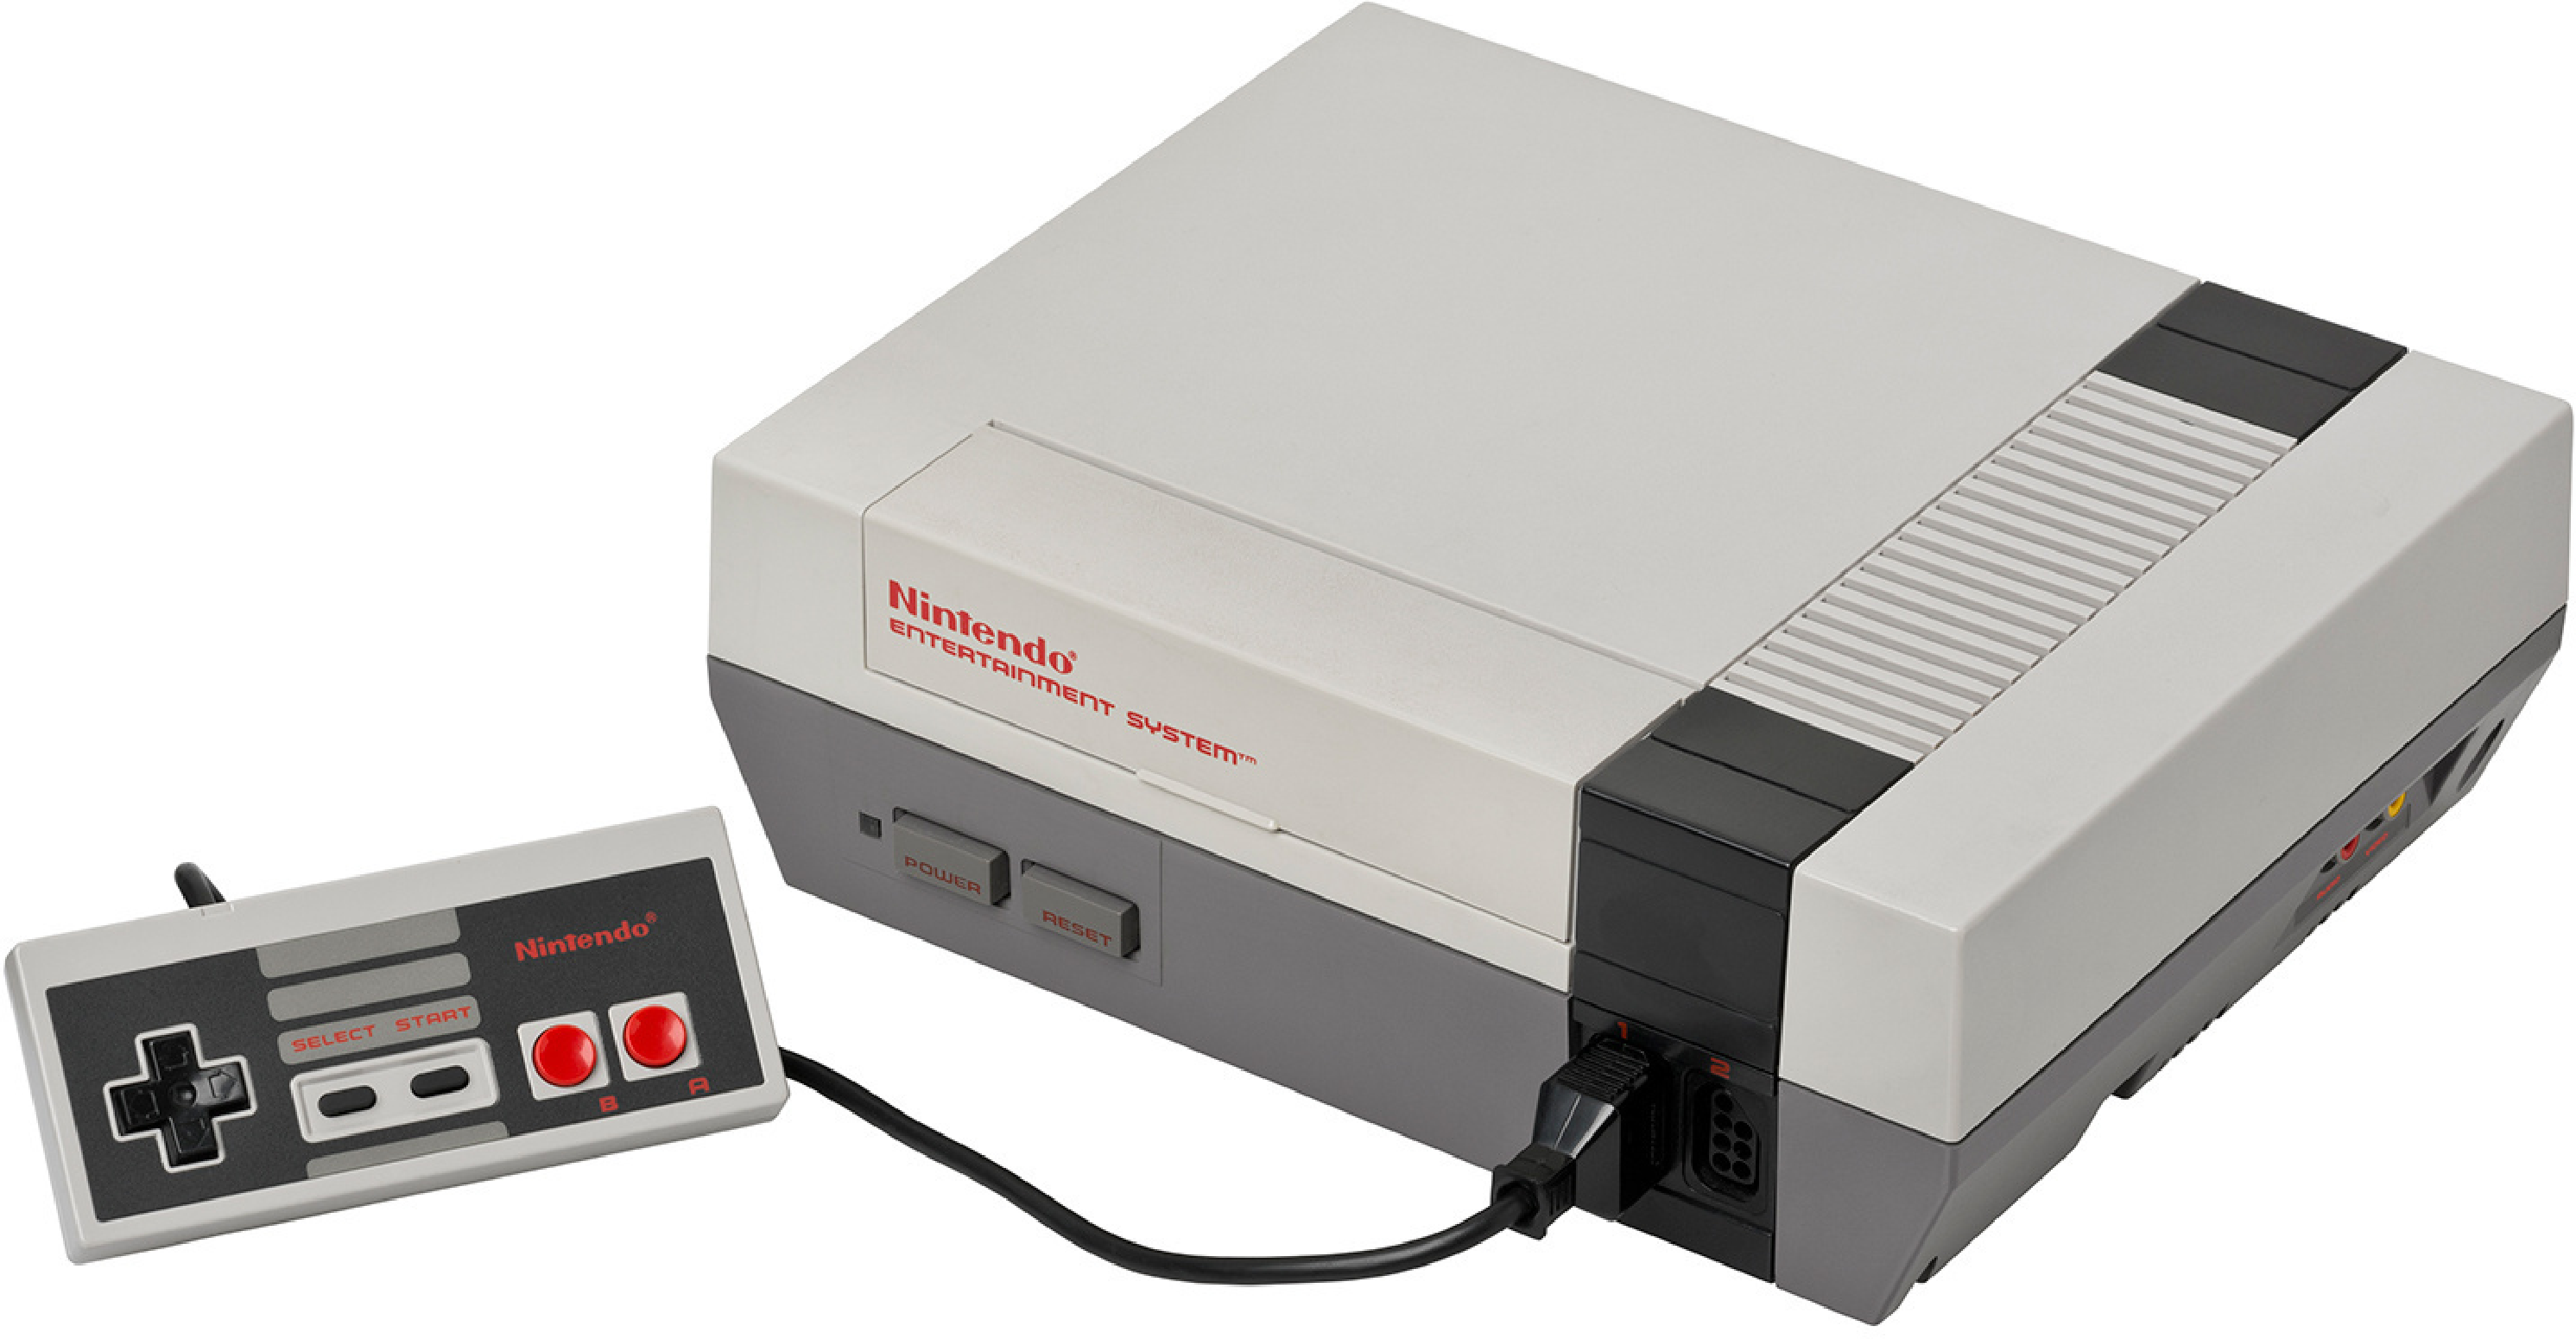
\includegraphics[height=70pt]{figures/nintendo-classic}
		\qquad
		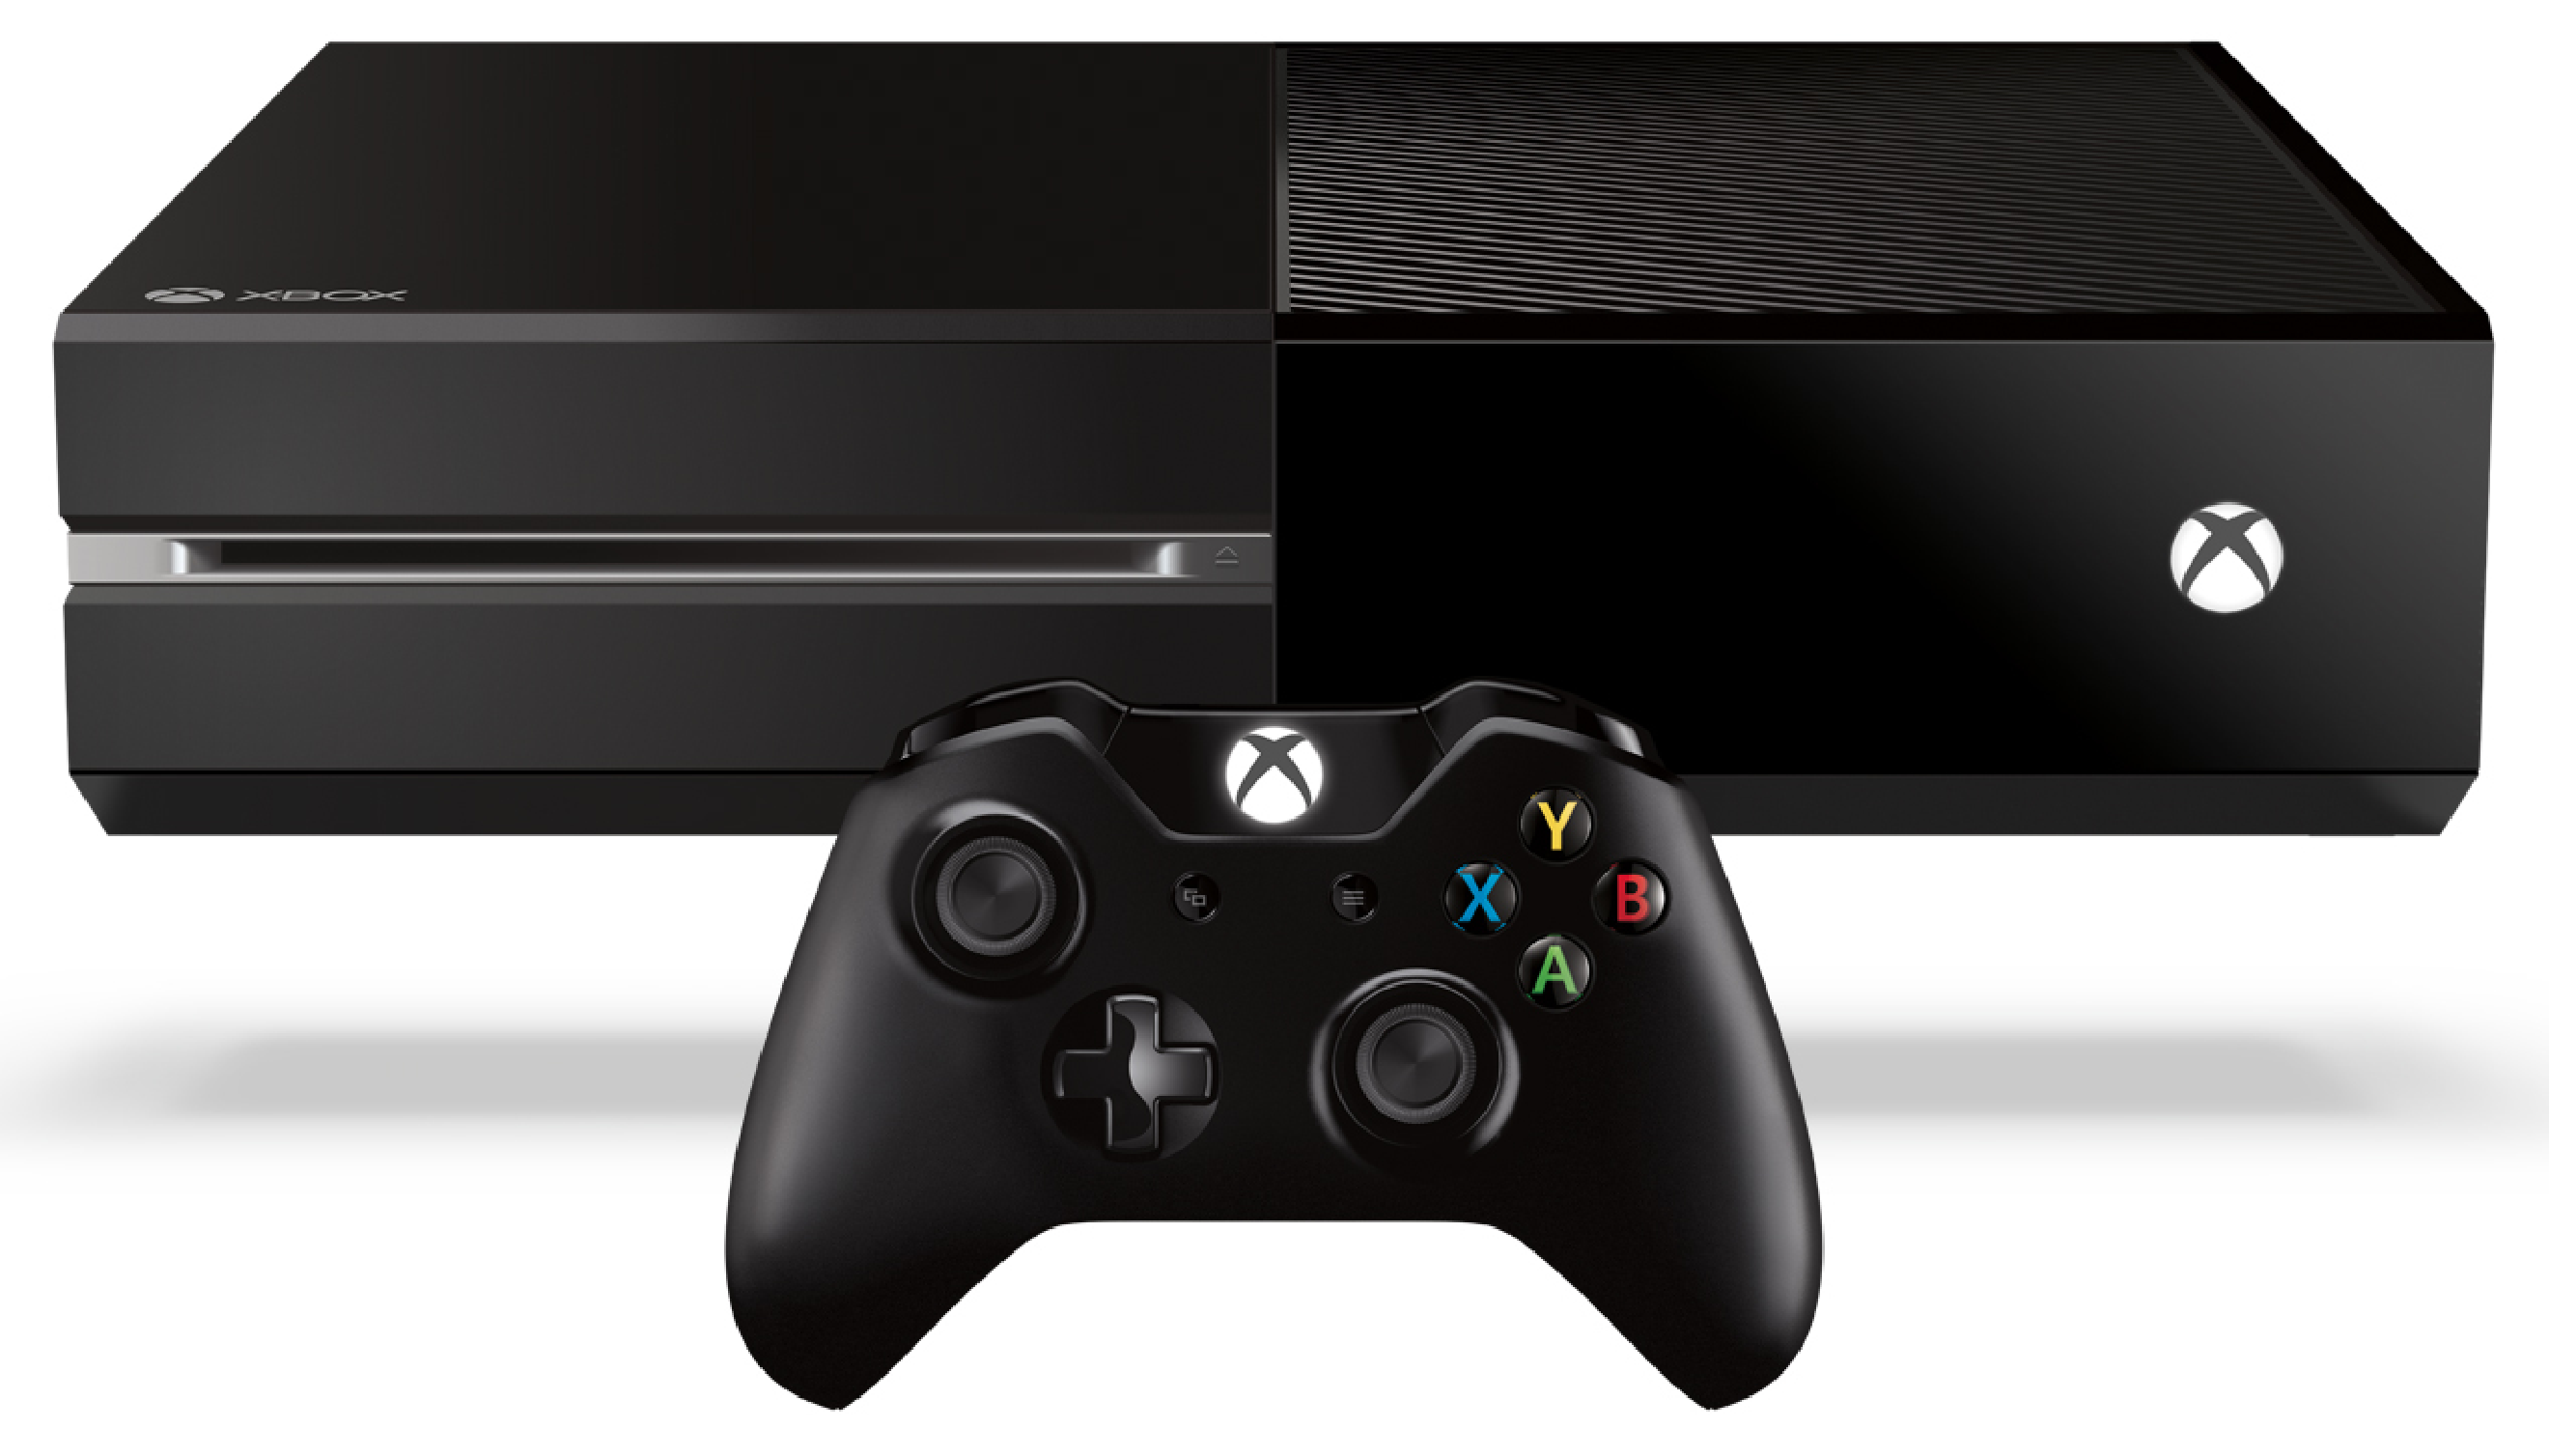
\includegraphics[height=70pt]{figures/xbox-one}
	\end{figure}
}

\end{frame}

\begin{frame}{Simulation Technologies}

Broadly, there are two software-based simulation technologies:

\bigskip

\centering
\begin{tabular}{l l l}
Technology & Slowdown & Complexity \\
\hline
Interpretation & 1000x & Low \\
\alert<2->{Binary Translation} & \alert<2->{10x} & \alert<2->{High} \\

\end{tabular}

\bigskip

\onslide<3>{Can we get the \alert{speed} of BT without the \alert{complexity}?}

\end{frame}

\begin{frame}[fragile]{Example QEMU Instruction}
\begin{lstlisting}[language=C]
target_long imm = sextract64(inst, 20,12);
int rs1 = extract32(inst, 15, 5);
int rd  = extract32(inst, 7, 5);
TCGv source1 = tcg_temp_new();
gen_get_gpr(source1, rs1);
tcg_gen_addi_tl(source1, source1, imm);
gen_set_gpr(rd, source1);
tcg_temp_free(source1);
\end{lstlisting}
\end{frame}

\subsection{Architecture Description Languages}

\begin{frame}
\frametitle{Architecture Description Languages}

ADLs are useful tools for systems development. They let us:
\begin{itemize}
	\item<2-> ...describe systems at different levels of abstraction
	\item<3-> ...use new technologies without rewriting all of our tools
	\item<4-> ...separate the behaviour of tools from their implementation
\end{itemize}

\bigskip

\centering
\onslide<2->{
	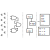
\includegraphics[width=0.25\textwidth]{figures/adl-levels-small}\qquad
}
\onslide<3->{
	
\includegraphics[width=0.25\textwidth]{figures/tool-portability}\qquad
}
\onslide<4->{
	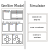
\includegraphics[width=0.25\textwidth]{figures/implementation-separation}
}

\end{frame}

\begin{frame}[fragile]{QEMU/ADL Comparison}
    \begin{minipage}{0.48\textwidth}
        \begin{lstlisting}[language=C,basicstyle=\tt\tiny,frame=single]
target_long imm = sextract64(inst, 20,12);
int rs1 = extract32(inst, 15, 5);
int rd  = extract32(inst, 7, 5);
TCGv source1 = tcg_temp_new();
gen_get_gpr(source1, rs1);
tcg_gen_addi_tl(source1, source1, imm);
gen_set_gpr(rd, source1);
tcg_temp_free(source1);
        \end{lstlisting}
        
    \end{minipage} %
    \quad %
    \begin{minipage}{0.47\textwidth}
\begin{lstlisting}[basicstyle=\tt\tiny,frame=single]
sint32 imm = inst.imm;
imm <<= 20;
imm >>= 20;

sint32 rs = read_register_bank(inst.rs1);

rs += imm;

write_register_bank(GPR, inst.rd, rs);
    \end{lstlisting}
    \end{minipage}
\end{frame}

\begin{frame}
\centering

\includegraphics{figures/comparison-chart}
\end{frame}

\begin{frame}
\frametitle{Architecture Description Languages}

We consider ADLs mostly in the context of simulation
\begin{itemize}
	\item Low level ADLs are more suited to detailed simulation
	\item More abstract ADLs are better suited to fast simulation
\end{itemize}

\centering
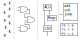
\includegraphics[width=0.8\textwidth]{figures/adl-levels}

\end{frame}


\section{GenSim}

\subsection{The GenSim ADL}

\begin{frame}{The GenSim ADL}

\end{frame}

\begin{frame}{The GenSim ADL}

GenSim is the name of our ADL toolset. It is designed to:

\begin{itemize}
	\item ... be intuitive and easy to learn
	\item ... create high performance simulation tools
	\item ... be extensible in terms of analyses

\end{itemize}

\end{frame}

\begin{frame}{GenSim Toolflow}

\centering
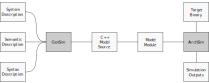
\includegraphics[width=\textwidth]{figures/gensim-toolflow}

\end{frame}

\begin{frame}{GenSim Model Components}

A GenSim description consists of three components
\pause

\begin{minipage}[h]{0.6\textwidth}
\begin{itemize}
\item A `System' component
\begin{itemize}
\item Available instruction sets
\item Register file layout
\item Configurable Features
\end{itemize}
\end{itemize}
\end{minipage}%
\begin{minipage}[h]{0.35\textwidth}
\centering
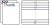
\includegraphics[width=\textwidth]{figures/component-system}
\end{minipage}

\smallskip
\pause

\begin{minipage}[h]{0.6\textwidth}
\begin{itemize}
\item A `Syntax' component
\begin{itemize}
\item Instruction formats
\item Instruction encoding
\end{itemize}
\end{itemize}
\end{minipage}%
\begin{minipage}[h]{0.35\textwidth}
\centering
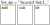
\includegraphics[width=\textwidth]{figures/component-syntax}
\end{minipage}

\smallskip
\pause

\begin{minipage}[h]{0.6\textwidth}
\begin{itemize}
\item A `Semantics' component
\begin{itemize}
\item Instruction behaviours
\item Exception behaviour
\end{itemize}
\end{itemize}
\end{minipage}%
\begin{minipage}[h]{0.35\textwidth}
\centering

\includegraphics[width=\textwidth]{figures/component-semantics}
\end{minipage}

\end{frame}

\begin{frame}{Available Models}

\centering
\begin{columns}
\begin{column}{0.6\textwidth}
\begin{itemize}
	\item ARMv7-A 
	\only<2>{
		\begin{itemize}
			\item ARM + Thumb-2
			\item Some VFP and NEON
			\item User Mode + Full System
		\end{itemize}
	}
	\item ARMv8
	\only<3>{
		\begin{itemize}
			\item AArch64 Only
			\item Some FP Support
			\item User Mode + Full System
		\end{itemize}
	}
	\item RISC-V
	\only<4>{
		\begin{itemize}
			\item Core and FP
			\item User Mode only
		\end{itemize}
	}
	\item x86-64
	\only<5>{
		\begin{itemize}
			\item External decoder
			\item User Mode only
		\end{itemize}
	}
\end{itemize}
\end{column}
\begin{column}{0.4\textwidth}

\only<2>{
\centering
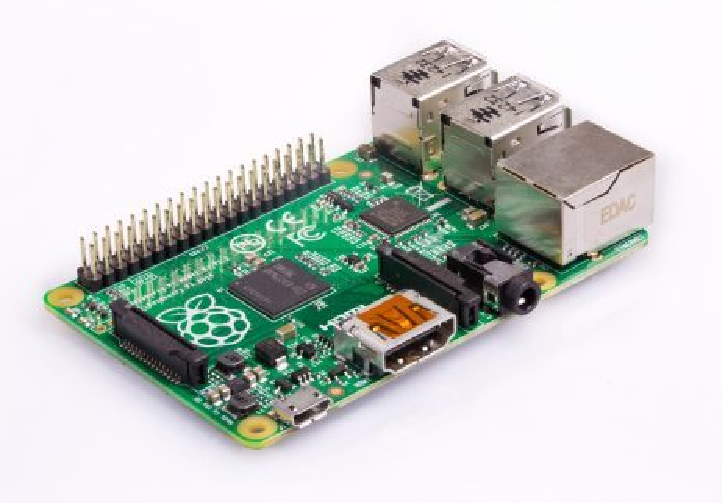
\includegraphics[width=\textwidth]{figures/rpi1}\\
\centering
\tiny{Raspberry Pi Model B}
}
\only<3>{
\centering
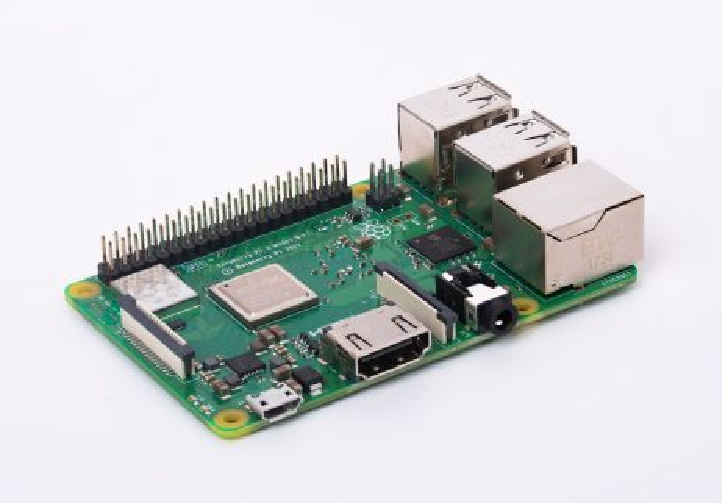
\includegraphics[width=\textwidth]{figures/rpi2}\\
\tiny{Raspberry Pi 3 Model B+}
}
\only<4>{
\centering
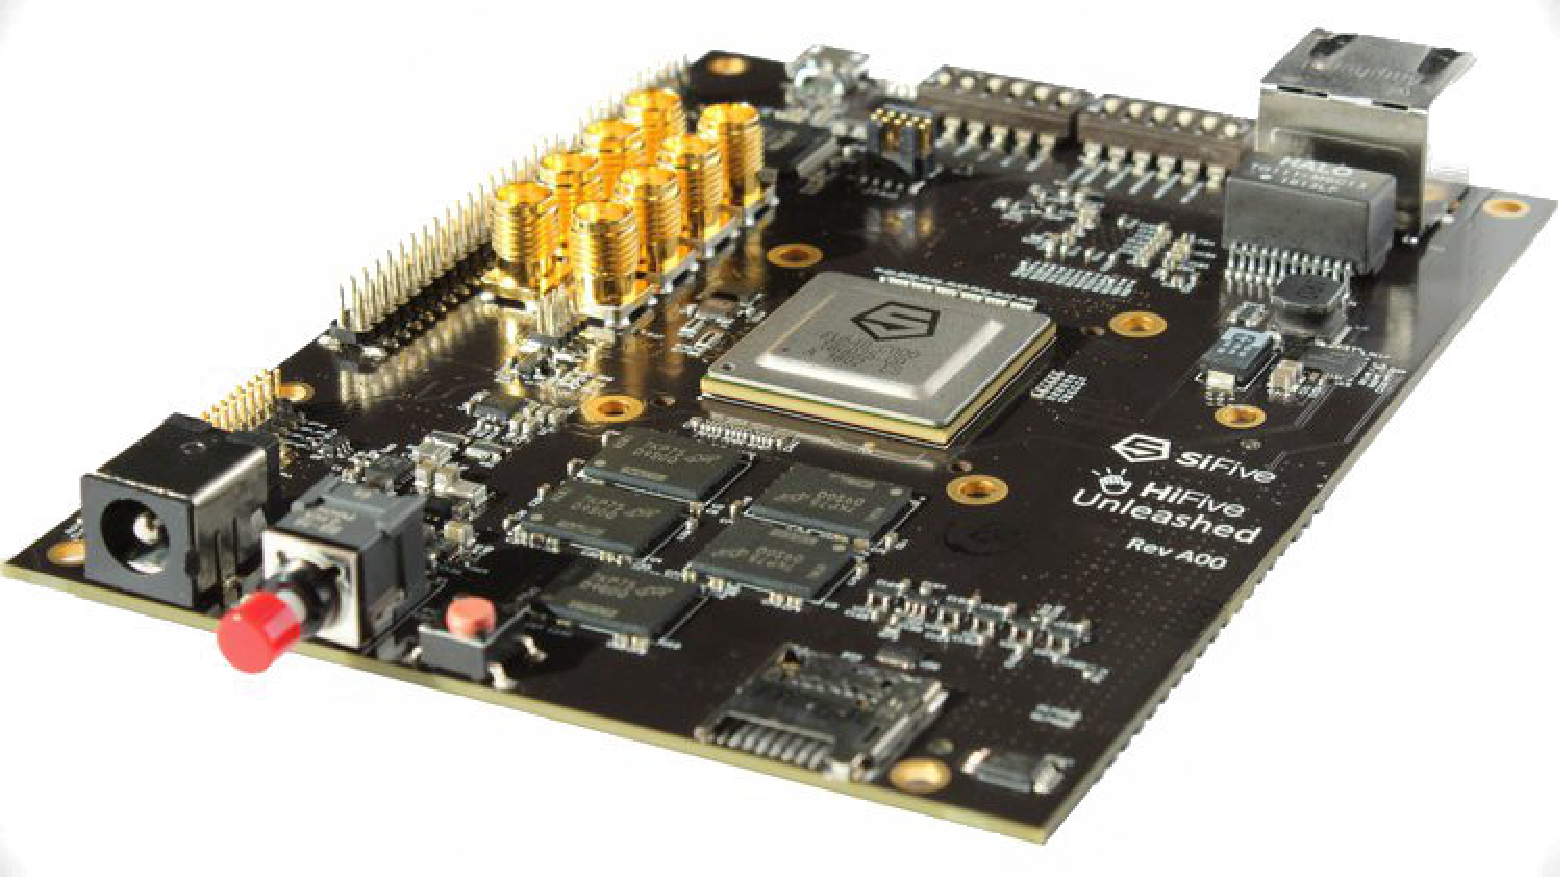
\includegraphics[width=\textwidth]{figures/riscv-sifive}\\
\tiny{SiFive RISC-V SBC}
}
\only<5>{
\centering
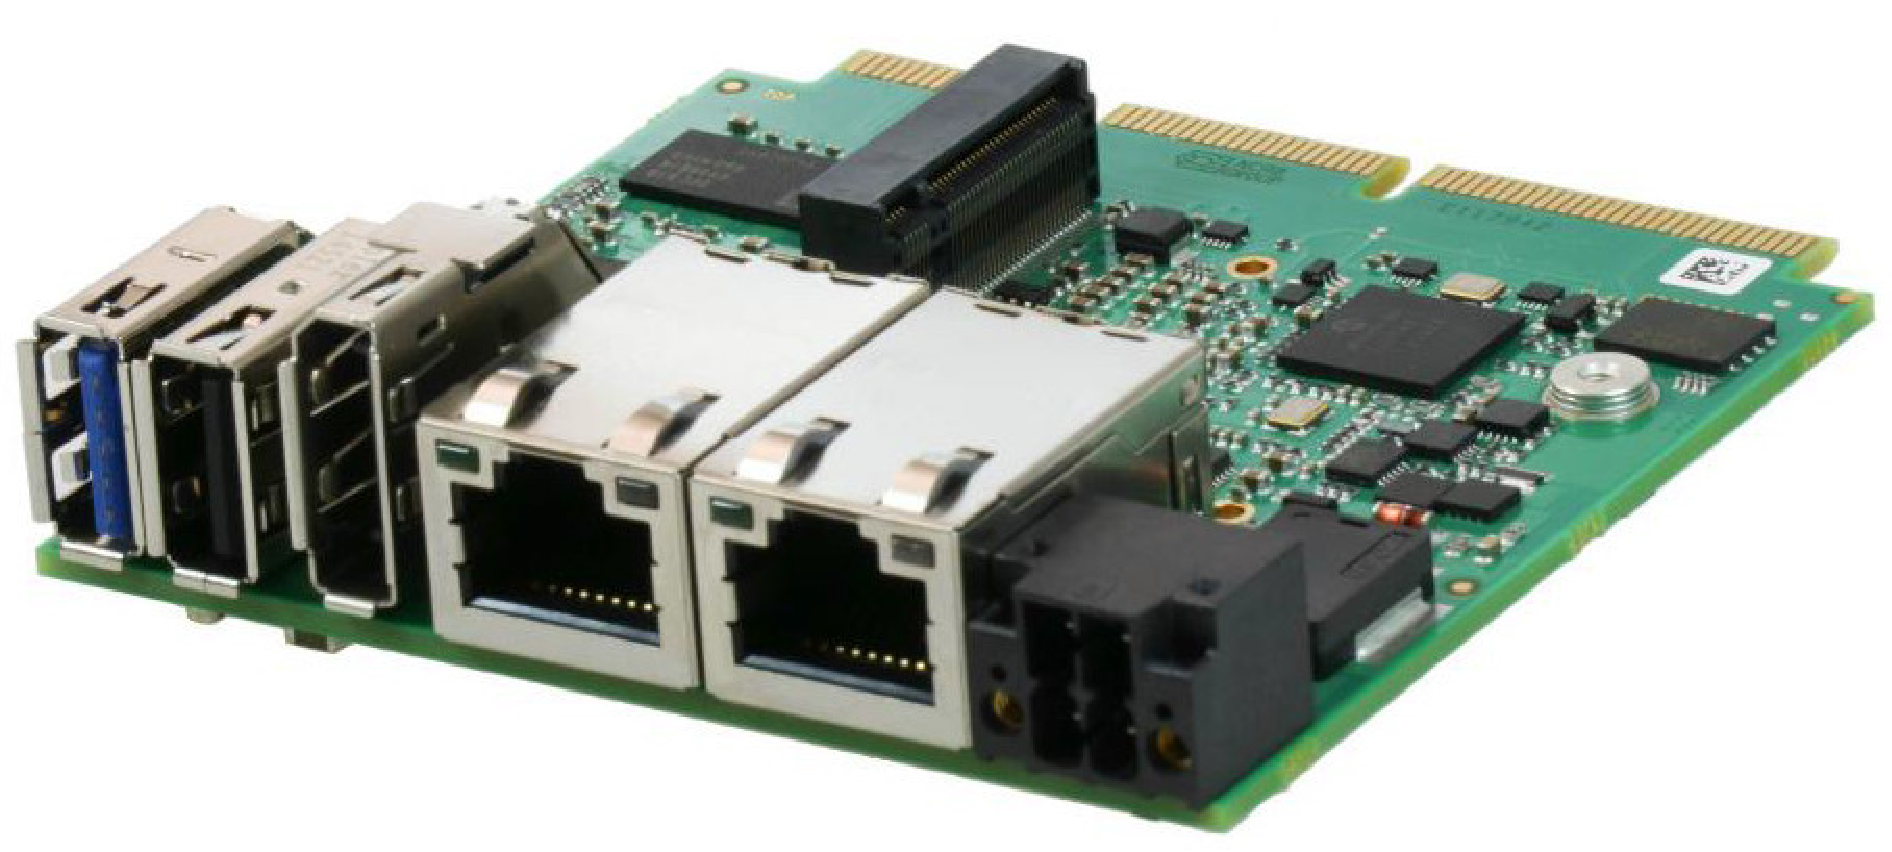
\includegraphics[width=\textwidth]{figures/x86-sbc}\\
\tiny{ADL ADLE3800SEC}
}

\end{column}
\end{columns}

\end{frame}

\begin{frame}{Execution Model}

\begin{minipage}[t][0.4\textheight]{\textwidth}
GenSim generally has a simplistic execution model
\begin{itemize}
	\item Instructions have a straightforward encoding
	\item Instructions are executed in PC order
	\item Effects occur immediately
	\item Instructions can be predicated
\end{itemize}
\end{minipage}

\pause

\begin{minipage}[t][0.4\textheight]{\textwidth}
Which architectures do not fit this model?
\begin{itemize}
	\item x86 (stateful encoding)
	\item MIPS (delay slots)
	\item DSP-like architectures (delayed effects)
\end{itemize}
\end{minipage}

\end{frame}

\subsection{The ArchSim Simulator}

\begin{frame}{The ArchSim Simulator}

\end{frame}

\begin{frame}{The ArchSim Simulator}

ArchSim is our research simulation platform. It is highly modular and configurable.

\begin{itemize}
	\item User Mode \& Full System Simulation
	\item Modular in terms of processors, devices, and platforms
	\item High speed trace system
\end{itemize}

\end{frame}

\begin{frame}{Simulation Modes}

User Mode Simulation
\begin{itemize}
	\item Run a single user mode application
	\item Emulate system calls (e.g. input/output)
\end{itemize}

\bigskip

Full System Simulation
\begin{itemize}
	\item Model a full system including external devices
	\item Some performance costs due to MMU translations
\end{itemize}

\end{frame}

\begin{frame}{Modularity}

ArchSim can accept a variety of modules
\begin{itemize}
	\item GenSim processor modules
	\item External devices
\end{itemize}

This allows devices to be developed as closed-source and still used
by ArchSim

% Processor modules from GenSim
% Accepts device modules
% (Used for closed-source GPU simulation)

\end{frame}

\begin{frame}{High Speed Tracing}

\begin{minipage}[h]{0.45\textwidth}
\begin{itemize}
	\item High performance (>1MIPS)
	\item Full architectural trace
	\item Easily extensible
	\item Tools for manipulation \\\& visualisation
\end{itemize}
\end{minipage} %
\begin{minipage}[h]{0.45\textwidth}
\centering
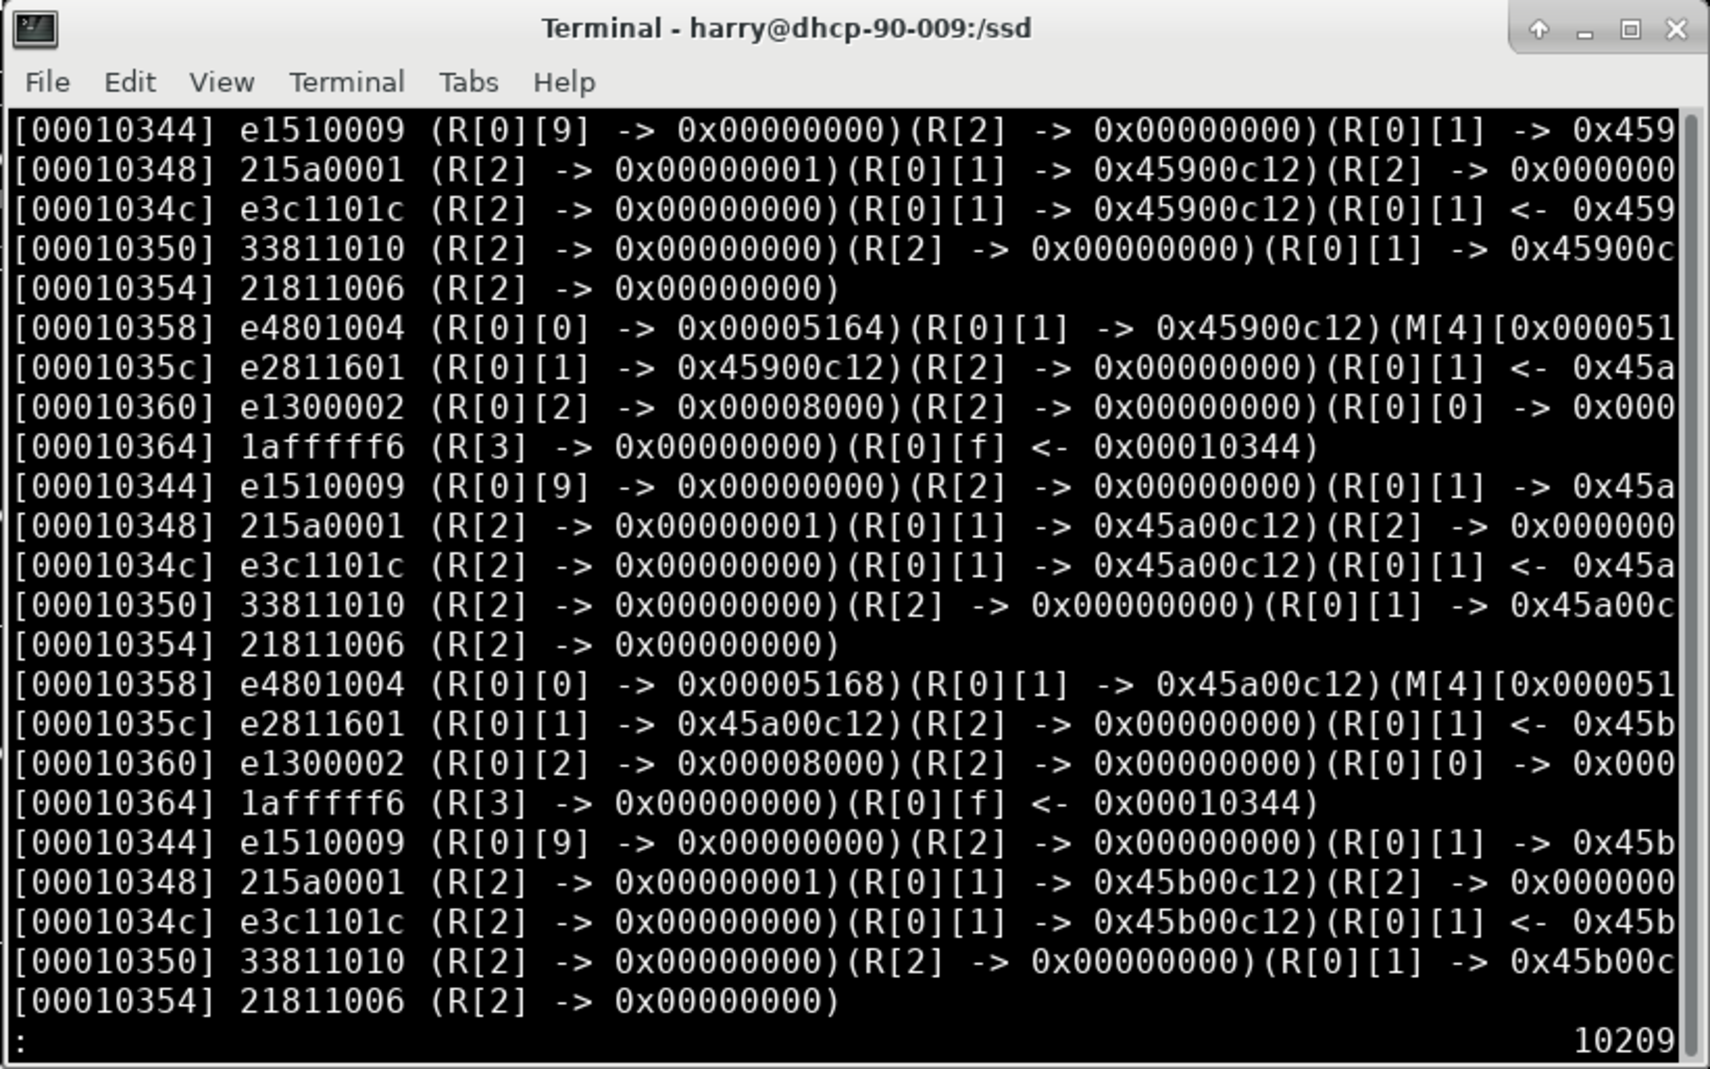
\includegraphics[width=\textwidth]{figures/trace}
\end{minipage}

\end{frame}

\begin{frame}{Short Demo}

(Video)

\end{frame}

\subsection{Captive}

\begin{frame}{The Captive Cross-Architectural Hypervisor}

\end{frame}

\begin{frame}{Captive}

\end{frame}

\begin{frame}{Captive}

Alternative simulation tool which uses GenSim ADL models

Uses host virtualisation features to improve simulation speed

\end{frame}

\begin{frame}{Captive}
	
	Not currently available (but coming soon!)
	
\end{frame}


\end{document}
